\begin{frame}
  \frametitle{Sparse Grids -- Implementation}
  \topline
  \vspace{-10px}
  \begin{block}{Computational efficient implementation}
    \begin{itemize}
    \item Tensor-product structure
    \item Nested structure
    \item Recursive, tree-like traversal
    \end{itemize}
  \end{block}
  \begin{block}{Problems}
    \begin{itemize}
    \item Scattered memory access patterns
    \item Inherently recursive, hard to parallelize
    \end{itemize}
  \end{block}
\end{frame}


\begin{frame}
  \frametitle{Sparse Grids -- Basics}
  \topline
  \vspace{-10px}
  \begin{block}{Hierarchical, nested structure}
    \begin{figure}[!htp]
      \setbeamertemplate{caption}{\raggedright\insertcaption\par}
      \setbeamerfont{caption}{size=\footnotesize}
      \centering
      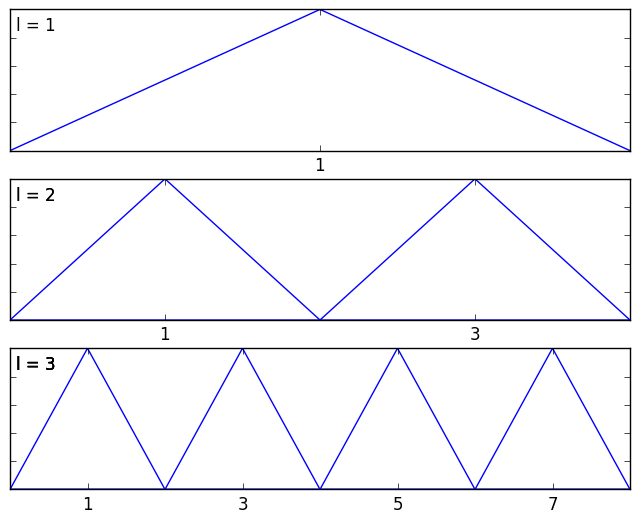
\includegraphics[width=7.5cm]{images/sparse_hats}
      \vspace{-12px}
      \caption{}
    \end{figure}
  \end{block}
\end{frame}


\begin{frame}
  \frametitle{Sparse Grids -- Implementation}
  \topline
  \vspace{-10px}
  \begin{block}{Iterative implementation}
    \begin{itemize}
    \item Disregards the hierarchical, nested structure
    \item Calculates $\phi_i(x^{(j)})$ for every $\phi_i$ and $x^{(j)}$
    \item 3 for-loops: data points, grid points, dimensions
    \end{itemize}
  \end{block}
  \begin{block}{Trade-off}
    \begin{itemize}
    \item Parallelization/Vectorization
    \item Linear memory access allowing pre-fetching
    \item Many (!) unnecessary computations (zero-evaluations)
    \end{itemize}
  \end{block}
\end{frame}


\begin{frame}
  \frametitle{Sparse Grids -- Implementation}
  \topline
  \vspace{-10px}
  \begin{block}{Hierarchical subspaces}
    \begin{figure}[!htp]
      \setbeamertemplate{caption}{\raggedright\insertcaption\par}
      \setbeamerfont{caption}{size=\footnotesize}
      \centering
      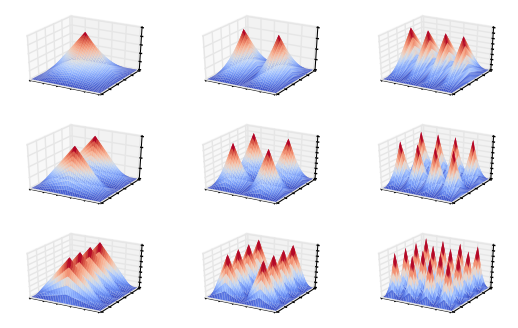
\includegraphics[width=7.5cm]{images/sparsegrid_2dhats}
      \vspace{-12px}
      \caption{}
    \end{figure}
  \end{block}
\end{frame}


\begin{frame}
  \frametitle{Summary}
  \topline
  \vspace{-10px}
  \begin{block}{Data mining with sparse grids}
    \begin{itemize}
    \item Discretization with hierarchical basis
    \item Sparseness and adaptivity
    \item Classification/Regression through least squares
    \item Iterative implementation to exploit parallelization
    \end{itemize}
  \end{block}
  \begin{block}{Conclusions}
    \begin{itemize}
    \item Linear scaling in the number of data points
    \item Mitigation of the curse of dimensionality
    \item Robust technique capable of dealing with non-linear data
    \end{itemize}
  \end{block}
\end{frame}


%%% Local Variables:
%%% TeX-master: "slides"
%%% End:
